% Cluster Computing (Springer Nature) — uses sn-jnl.cls v3.1 (Dec 2024)
% Template: https://www.springernature.com/gp/authors/campaigns/latex-author-support
\documentclass[pdflatex,sn-mathphys-num]{sn-jnl}

\usepackage{amsmath,amssymb,amsfonts}%
\usepackage{amsthm}%
\usepackage{mathrsfs}%
\usepackage{graphicx}%
\graphicspath{{./}{../}}
\usepackage{textcomp}%
\usepackage{xcolor}%
\usepackage{booktabs}%
\usepackage{multirow}%
\usepackage{algorithm}%
\usepackage{algorithmic}%
\usepackage{subcaption}%
\PassOptionsToPackage{hyphens}{url}\usepackage{url}%
\tolerance=2000
\emergencystretch=3em
\hbadness=10000

\theoremstyle{thmstyleone}%
\newtheorem{theorem}{Theorem}%
\newtheorem{proposition}{Proposition}%
\newtheorem{lemma}[theorem]{Lemma}%
\theoremstyle{thmstyletwo}%
\newtheorem{remark}{Remark}%
\theoremstyle{thmstylethree}%
\newtheorem{definition}{Definition}%
\raggedbottom

\newcommand{\mmonererr}{6.5}
\newcommand{\mmonererrA}{15.0}
\newcommand{\mmonererrB}{12.6}
\newcommand{\mmonererrC}{6.5}

\begin{document}

\title[GPU-MLMC Network Congestion]{GPU-Accelerated Multilevel Monte Carlo for Network
Congestion Propagation: Coupled SDE Models with Uncertainty Quantification}

\author[1]{\fnm{Paritosh} \sur{Dwivedi}}\email{paritosh.dwivedi2024@vitstudent.ac.in}
\author*[1]{\fnm{Anindita} \sur{Kundu}}\email{anindita.kundu@vit.ac.in}

\affil*[1]{\orgdiv{School of Computer Science and Engineering},
  \orgname{Vellore Institute of Technology},
  \orgaddress{\city{Vellore}, \postcode{632014}, \country{India}}}

\abstract{Internet service providers must provision capacity under uncertain demand while
keeping delay service-level agreements credible during bursts, failures, and diurnal load
changes. Deterministic planning and fixed safety margins either waste capacity or hide
violation risk. This paper presents a GPU-accelerated Multilevel Monte Carlo (MLMC)
framework that turns stochastic congestion models into confidence intervals and tail-delay
estimates for such provisioning decisions. The framework combines a coupled network diffusion
model with GPU-parallel sampling, so neighbouring queues can share congestion effects while
thousands of paths are simulated concurrently. MLMC reaches the target accuracy with order
$\varepsilon^{-2}$ work, whereas single-level Monte Carlo requires order $\varepsilon^{-3}$
work under the same SDE discretization assumptions. On identical A100 GPU hardware, GPU-MLMC
achieves up to 12.91$\times$ runtime speedup and 257.72$\times$ work reduction over
single-level GPU-MC at $\varepsilon=0.01$. The implementation exceeds 65,000 samples/s on
100-node networks, sustains practical throughput on 500-node topologies, and estimates
P95/P99 tail delay with $<0.2\%$ relative error against a tight Monte Carlo reference
(MLMC convergence accuracy). Cross-validation of the underlying SDE model against a Poisson
G/D/1 discrete-event reference on MAWI backbone traffic shows that a time-varying CIR
diffusion coefficient $\sigma(t){=}\sqrt{\lambda(t)}$ reduces the median SDE--DES tail
discrepancy to $7.1\%$ on P95 and $7.0\%$ on P99---only $2.1$ percentage points above the
finite-sample estimator floor---confirming distributional parity with the Poisson reference
at standard binning resolution.}

\keywords{Monte Carlo methods, GPU computing, network modeling, uncertainty quantification,
stochastic differential equations, queueing networks}

\maketitle

\section{Introduction}

Network traffic is stochastic at the time scales where service-level agreements
are won or lost: arrivals fluctuate, service rates vary, and correlated bursts can move delay risk
across adjacent links \cite{kelly2011stochastic,whitt2002,cisco2023annual}. Deterministic traffic
models compress this uncertainty into a single forecast, while ad-hoc provisioning margins give
operators little control over the probability or severity of SLA violations. As a result, an ISP
planning capacity for tail-delay guarantees must either overbuy infrastructure or accept
unquantified congestion risk.

This paper combines Multilevel Monte Carlo (MLMC), introduced by Heinrich
\cite{heinrich2001multilevel} and developed for SDE path simulation by Giles
\cite{giles2008multilevel}, with GPU parallelism for network congestion uncertainty
quantification. MLMC reduces the number of fine-resolution paths needed for a target accuracy,
and GPUs execute the remaining path ensemble concurrently. We deliver a coupled SDE congestion
model, a GPU-MLMC estimator, and empirical validation on synthetic and CAIDA topology subgraphs.
Our key contributions are: (1)~a \emph{coupled} SDE model for network-wide congestion
propagation ($dC_i = (\sum_j \alpha_{ij}C_j - \beta_i C_i)dt + \sigma_i dW_i$) with
degree-normalised influence weights \cite{kang2007,harrison1985}, integrated into the
GPU-MLMC estimation loop to enable correlated uncertainty quantification across neighbouring
nodes; (2)~an adaptive MLMC implementation with optimal sample allocation and a crossover
model characterising when MLMC runtime advantage emerges over single-level GPU-MC
\cite{giles2015multilevel,collier2015}; (3)~\emph{Adaptive Network-Aware MLMC} (ANA-MLMC),
a new sample-allocation rule that minimises a centrality-, pilot-variance-, and
SLA-priority-weighted estimator variance
(Eqs.~\eqref{eq:ana_var}--\eqref{eq:ana_weights}), preserves
$\mathcal{O}(\varepsilon^{-2})$ complexity, and concentrates effort on operationally
consequential nodes; and (4)~empirical validation on synthetic Erd\H{o}s-R\'enyi,
Barabasi-Albert, and real-world CAIDA AS-rel2 topologies ($n=500$).

\section{Related Work}

\subsection{MLMC and SDE Numerics}

The Euler-Maruyama scheme provides the foundation for numerical integration of SDEs
\cite{kloeden1992}, with weak order 1 and strong order 0.5 for Lipschitz coefficients
\cite{khasminskii2012}. MLMC was developed for parametric integration
\cite{heinrich2001multilevel} and SDE path simulation \cite{giles2008multilevel}, and has since
been extended to computational finance \cite{giles2012finance,glasserman2003monte}, fluid
dynamics \cite{mishra2012sparse}, elliptic PDEs \cite{cliffe2015}, and Bayesian inference
\cite{dodwell2015hierarchical}. Key theoretical results establish $\mathcal{O}(\varepsilon^{-2})$
complexity when variance decays as $\mathcal{O}(2^{-\alpha l})$ and cost grows as
$\mathcal{O}(2^{\gamma l})$ with $\alpha \geq \frac{1}{2}\gamma$ \cite{giles2015multilevel}.
Recent surveys cover MLMC in finance \cite{giles2024review} and small-noise SDE settings
\cite{spiliopoulos2022multilevel} relevant to our low-diffusivity regime.

\subsection{GPU Monte Carlo and Network Queueing Models}

%ADDED BY AK
\begin{sidewaystable}[p]
%\caption{GPU-Accelerated Monte Carlo Methods in Literature and Network Congestion Modeling Approaches}
\captionof{table}{GPU-Accelerated Monte Carlo Methods in Literature}
\label{tab:gpu_lit}
\begin{tabular}{llllccll}
\toprule
Work & Reference & Domain & GPU & MLMC? & Net.-aware? &
Net.-scale Valid.? & Tail UQ? \\
\midrule
CPU MLMC & Giles \cite{giles2008multilevel} & SDE finance & No & Yes & No & No & No \\
GPU MC (Ising) & Preis et al.\ \cite{thompson2010gpu} & Stat.\ Physics & Yes & No & No & No & No \\
GPU Computing & Owens et al.\ \cite{owens2008} & General GPU & Yes & No & No & No & No \\
CUDA Reduction & Harris et al.\ \cite{harris2007} & HPC & Yes & No & No & No & No \\
GPU Particle & Bergmann et al.\ \cite{bergmann2017gpu} & Physics & Yes & No & No & No & No \\
GPU Network Sim & Sha et al.\ \cite{sha2023gpu} & Networking & Yes & No & No & Partial & No \\
Neural MC Traffic & Chen et al.\ \cite{chen2022neural} & Networking & Yes & No & No &
Yes (surrogate) & No \\
Proposed Work & This work & Network UQ & Yes & Yes & Yes & Yes (real-topology) & Yes \\
\bottomrule
\end{tabular}

\vspace{1cm} % vertical space between tables
\captionof{table}{Network Congestion Modeling Approaches}
\label{tab:network_modeling}
\begin{tabular}{lllll}
\toprule
Approach & Reference & UQ Support & Tail Delay & Scalability \\
\midrule
Stochastic Networks Theory & Kelly \cite{kelly2011stochastic} & Theoretical & Limited & Analytical \\
Heavy-Traffic Diffusion & Whitt \cite{whitt2002} & Theoretical & Analytical & Not scalable \\
Reflected Brownian Motion & Harrison \cite{harrison1985} & Theoretical & Analytical & Not sim.-focused \\
Event-Driven Simulation & OMNeT++/ns-3 \cite{perumalla2011discrete} & None & None & High-fidelity; no UQ \\
Proposed MLMC-GPU & This work & Full distribution & P95, P99, CI & Real-topology validated \\
\bottomrule
\end{tabular}
\vspace{1cm}
\captionof{table}{Algorithmic Complexity Comparison for Stochastic SDE Simulation}
\label{tab:complexity}
\begin{tabular}{llllcl}
\toprule
Method & Core Reference & Problem Domain & Total Cost ($\varepsilon$ target) &
Var.\ Reduction & Applicability \\
\midrule
Standard Monte Carlo & Glasserman \cite{glasserman2003monte} & SDE simulation &
$\mathcal{O}(\varepsilon^{-3})$ & No & Generic \\
MLMC (CPU) & Giles \cite{giles2008multilevel,giles2015multilevel} & SDE simulation &
$\mathcal{O}(\varepsilon^{-2})$ & Yes & Generic \\
Proposed MLMC + GPU & This work & Network congestion SDE &
$\mathcal{O}(\varepsilon^{-2})$ (parallelized) & Yes & Real-topology validated \\
\bottomrule
\end{tabular}


\end{sidewaystable}

Stochastic network models based on queueing theory provide mathematical foundations for
performance analysis \cite{kelly2011stochastic,whitt2002}. Diffusion approximations enable
continuous-time modeling of discrete queueing systems \cite{kang2007,harrison1985}. Roy et al.\
\cite{roy2016} extend these models to semi-open networks. Recent work incorporates SDEs to model
time-varying arrival and service rates \cite{mandelbaum2014stochastic}. Network propagation
phenomena on random graphs \cite{hofstad2016} and epidemic models \cite{kenah2011} share similar
mathematical structure. Large deviation theory provides tools for rare event analysis
\cite{chatterjee2017}. Table~\ref{tab:network_modeling} summarizes how these theoretical models
compare with the proposed simulation-oriented MLMC-GPU framework.

\section{Methodology}

\subsection{SDE-Based Network Model}

We model network queue dynamics using a stochastic differential equation that captures both mean
behavior and random fluctuations \cite{kloeden1992,khasminskii2012}:

\begin{equation}
    dQ(t) = (\lambda(t) - \mu(t))dt + \sigma dW(t)
    \label{eq:sde}
\end{equation}

\noindent where $Q(t)$ is the queue length, $\lambda(t)$ is the arrival rate, $\mu(t)$ is the
service rate, $\sigma$ controls noise magnitude, and $W(t)$ is a standard Wiener process. This
diffusion approximation is justified by classical heavy-traffic limit theorems for queueing
networks \cite{kang2007,whitt2002}.

For numerical integration, we use the Euler-Maruyama scheme with time step $h$
\cite{kloeden1992}:

\begin{equation}
    Q_{n+1} = Q_n + (\lambda_n - \mu_n)h + \sigma\sqrt{h}Z_n
    \label{eq:euler}
\end{equation}

\noindent where $Z_n \sim \mathcal{N}(0,1)$ are independent standard normal random variables.
Reflecting boundary conditions at $Q=0$ ensure non-negativity, consistent with reflected Brownian
motion models for queueing systems \cite{harrison1985}.

\par\noindent\textbf{Time-varying CIR diffusion.}
For bursty Poisson arrivals the constant-$\sigma$ assumption under-estimates per-step variance at
low-rate intervals and over-estimates it during bursts. We therefore introduce a
\emph{time-varying} diffusion coefficient $\sigma(t)=\sqrt{\lambda(t)}$, the
Cox--Ingersoll--Ross square-root-diffusion regime \cite{kang2007}, which exactly matches the
per-step standard deviation of $\mathrm{Poisson}(\lambda(t)\,dt)$ arrivals. The discrete update
becomes
\begin{equation}
    Q_{n+1} = \max\!\bigl(0,\; Q_n + (\lambda_n - \mu)\,h + \sqrt{\lambda_n\,h}\;Z_n\bigr),
    \label{eq:tv_sigma}
\end{equation}
where $Z_n \sim \mathcal{N}(0,1)$.  No free parameters are introduced: $\sigma(t)$ is fully
determined by the observed arrival trace. Real-trace validation
(Section~\ref{subsec:mawi_validation}) shows this reduces the SDE--DES discrepancy to
distributional parity with the Poisson reference.

\subsection{Multilevel Monte Carlo}

The MLMC estimator combines samples from multiple resolution levels to achieve variance reduction
\cite{giles2008multilevel,giles2015multilevel}. Let $P_l$ denote the quantity of interest
computed at level $l$ with time step $h_l = h_0 \cdot 2^{-l}$. The MLMC estimator is:

\begin{equation}
    \hat{Y} = \sum_{l=0}^{L} \frac{1}{N_l} \sum_{i=1}^{N_l} (P_l^{(i)} - P_{l-1}^{(i)})
    \label{eq:mlmc}
\end{equation}

\noindent where $P_{-1} \equiv 0$ and $P_l^{(i)}, P_{l-1}^{(i)}$ are computed using the same
random path (coupling).

The optimal sample allocation that minimizes variance for a fixed computational budget is given
by the Giles formula \cite{giles2015multilevel}:

\begin{equation}
    N_l^* \propto \sqrt{\frac{V_l}{C_l}}
    \label{eq:giles}
\end{equation}

\noindent where $V_l = \text{Var}[P_l - P_{l-1}]$ is the level variance and $C_l$ is the cost
per sample at level $l$.

For SDEs with Lipschitz coefficients, the weak error is $\mathcal{O}(h_l)$ and the variance
decays as $V_l = \mathcal{O}(h_l) = \mathcal{O}(2^{-l})$, yielding optimal
$\mathcal{O}(\varepsilon^{-2})$ complexity \cite{giles2015multilevel,higham2015}. Adaptive
methods \cite{collier2015} can further improve efficiency.
Table~\ref{tab:complexity} highlights the complexity-positioning of standard MC, classical MLMC,
and our MLMC + GPU implementation.

%Blocked by AK
%\begin{sidewaystable}[tp]
%\caption{Algorithmic Complexity Comparison for Stochastic SDE Simulation}
%\label{tab:complexity}
%\begin{tabular}{llllcl}
%\toprule
%Method & Core Reference & Problem Domain & Total Cost ($\varepsilon$ target) &
%Var.\ Reduction & Applicability \\
%\midrule
%Standard Monte Carlo & Glasserman \cite{glasserman2003monte} & SDE simulation &
%$\mathcal{O}(\varepsilon^{-3})$ & No & Generic \\
%MLMC (CPU) & Giles \cite{giles2008multilevel,giles2015multilevel} & SDE simulation &
%$\mathcal{O}(\varepsilon^{-2})$ & Yes & Generic \\
%Proposed MLMC + GPU & This work & Network congestion SDE &
%$\mathcal{O}(\varepsilon^{-2})$ (parallelized) & Yes & Real-topology validated \\
%\bottomrule
%\end{tabular}
%\end{sidewaystable}
%Blocked by AK

\subsection{Single-Level GPU Monte Carlo Baseline}

For fair comparison, we implement a single-level GPU Monte Carlo (GPU-MC) baseline using
Euler--Maruyama discretization at the finest timestep $h_L$. This corresponds to the classical
Monte Carlo approach described in \cite{glasserman2003monte} with GPU parallelization following
standard CUDA practices \cite{nvidia2020cuda,owens2008,harris2007}. No multilevel correction
is applied. Equal-accuracy comparison is enforced via matched confidence interval half-widths.

\subsection{GPU Parallelization Strategy}

Our GPU implementation parallelizes across independent Monte Carlo samples using CUDA~\cite{nvidia2020cuda}: each thread executes a complete SDE path simulation with shared noise for fine/coarse coupling. Key optimizations include coalesced memory access, shared-memory reduction~\cite{harris2007}, and asynchronous kernel launches for level pipelining.

Table~\ref{tab:cpu_baselines} summarises single-thread and multi-core CPU baselines measured on
the same host as the A100 pod, providing context for the CPU-to-GPU speedup figures cited in the
abstract.

\begin{table}[!t]
\caption{CPU Baseline Throughput (Intel Xeon, synthetic $n{=}500$,
         $N{=}10{,}000$ samples)}
\label{tab:cpu_baselines}
\centering
\begin{tabular}{@{}l c c c@{}}
\toprule
Baseline & Cores & Throughput (samples/s) & GPU Speedup$^\dagger$ \\
\midrule
CPU single-thread (NumPy) & 1  & $\sim$200   & 87--644$\times$ \\
CPU multi-core (joblib)   & 8  & $\sim$1{,}400 & 12--90$\times$  \\
GPU A100 (this work)      & -- & $>$100{,}000 & 1$\times$ (ref) \\
\bottomrule
\end{tabular}
\vspace{2pt}
\footnotesize
$^\dagger$Speedup relative to each CPU baseline; values are
approximate and depend on sample count and network size.
\end{table}

\subsection{Coupled Congestion Propagation SDE}
\label{subsec:spatial}

The per-node scalar SDE model (Eq.~\eqref{eq:sde}) treats queue dynamics independently at each
node. We extend this to a \emph{coupled} network-wide congestion propagation model
\cite{kang2007,harrison1985,mandelbaum2014stochastic}:

\begin{equation}
    dC_i(t) = \left(\sum_j \alpha_{ij} C_j(t) - \beta_i C_i(t)\right)dt
              + \sigma_i\, dW_i(t)
    \label{eq:coupled_sde}
\end{equation}

\noindent where $\alpha_{ij} = \alpha \cdot A_{ij} / \deg(i)$ is the degree-normalised influence
of neighbour $j$ on node $i$ (derived from the adjacency matrix $A$), and $\beta_i$ is a per-node
congestion decay rate. Each Euler--Maruyama step evaluates the full $n \times n$ matrix-vector
product $A\mathbf{C}$ in a single PyTorch \texttt{torch.mv} call on the GPU, making the coupled
model as amenable to GPU parallelism as the per-node model.

For MLMC, coupled fine and coarse paths share the same Wiener increments $dW_i^{(k)}$ at each
step: fine steps use $\sqrt{h_l}$ increments while coarse steps sum pairs
$\sqrt{h_{l-1}} = \sqrt{2h_l}$, preserving the antithetic coupling required for variance
reduction. The \path{CongestionPropagationSDE.simulate_coupled_paths()} method implements this
scheme, and \path{GPUCoupledPropagationMLMC} integrates it into the GPU-MLMC estimation loop
. Experimental results showing correlated queue dynamics across
network nodes are presented in Section~V-D.

\subsection{Adaptive Network-Aware MLMC (ANA-MLMC)}
\label{subsec:ana_mlmc}

Standard MLMC sample allocation~\cite{giles2015multilevel} minimises the \emph{uniform}
estimator variance $\sum_l V_l/N_l$, treating every node in the network as equally important.
In a network operations setting this is rarely the right objective: an ISP cares more about queue
dynamics on high-betweenness backbone routers, peering links bound to strict SLAs, and nodes
whose pilot variance suggests sustained tail-risk. We propose \emph{Adaptive Network-Aware MLMC}
(ANA-MLMC), a sample allocation rule that explicitly carries this prioritisation through the MLMC
variance accounting.

\paragraph{Weighted variance criterion.}
Let $V_{l,i} = \mathrm{Var}\bigl(P_l^{(i)} - P_{l-1}^{(i)}\bigr)$ denote the per-node
level-difference variance and let $w \in \Delta^{n-1}$ be a vector of non-negative node weights
summing to one. ANA-MLMC defines the weighted level variance
\begin{equation}
    V_l^{w} \;=\; \sum_{i=1}^{n} w_i\, V_{l,i},
    \label{eq:ana_var}
\end{equation}
and minimises the weighted total estimator variance $\sum_l V_l^{w}/N_l$ subject to a fixed cost
budget $\sum_l N_l C_l \le B$. Standard Lagrangian analysis (analogous
to~\cite{giles2015multilevel}) yields the closed-form optimum
\begin{align}
    N_l^{\star} &\;\propto\; \sqrt{V_l^{w}/C_l}, \nonumber \\
    N_l &= \left\lceil \tfrac{2}{\varepsilon^{2}}\,
    \sqrt{V_l^{w}/C_l}\, \sum_k \sqrt{V_k^{w} C_k} \right\rceil .
    \label{eq:ana_giles}
\end{align}
\begin{sloppypar}
When $w_i = 1/n$, $V_l^{w}$ collapses to the standard uniform-mean variance and
Eq.~\eqref{eq:ana_giles} reduces \emph{exactly} to the Giles formula; a regression test
enforces this in the implementation.
\end{sloppypar}

\paragraph{Network-aware weight construction.}
We compose the weights from three normalised components:
\begin{equation}
    w_i \;=\; \mathrm{norm}\bigl(\gamma_C\, c_i
                + \gamma_V\, v_i^{\text{pilot}}
                + \gamma_S\, s_i\bigr),
    \label{eq:ana_weights}
\end{equation}
with $\gamma_C+\gamma_V+\gamma_S=1$ (defaults $0.4, 0.4, 0.2$). Here $c_i$ is PageRank centrality, $v_i^{\text{pilot}}$ the per-node pilot variance, and $s_i$ an optional SLA-priority vector (uniform if absent). Components are $\ell_1$-normalised so $w$ remains in the simplex.

\paragraph{Consistency and complexity.}
ANA-MLMC modifies only sample allocation, not the telescoping sum, so consistency and $\mathcal{O}(\varepsilon^{-2})$ complexity are inherited from standard MLMC; the per-level overhead is one additional $O(n)$ weighted reduction.


\subsection{Complexity Guarantees}
\label{subsec:complexity}

We formalise this as a theorem following Giles~\cite{giles2015multilevel}; network-risk weights enter only through a multiplicative constant.

\begin{theorem}[ANA-MLMC complexity]
\label{thm:complexity}
Assume the standard MLMC decay exponents $\alpha, \beta, \gamma > 0$: the level-difference
variance $V_l = \mathrm{Var}[P_l - P_{l-1}] = \mathcal{O}(2^{-\alpha l})$, the weak error
$|\mathbb{E}[P_l - P]| = \mathcal{O}(2^{-\beta l})$, and the cost per sample
$C_l = \mathcal{O}(2^{\gamma l})$, in the sense of~\cite{giles2015multilevel}.
For any fixed weight vector $\mathbf{w}$ with $w_i \ge 0$ and $\sum_i w_i = 1$,
the weighted level variance $V_l^w = \sum_i w_i V_{l,i}$ satisfies
$V_l^w = \mathcal{O}(2^{-\alpha l})$ (since $\sum_i w_i = 1$ and each $V_{l,i} = \mathcal{O}(2^{-\alpha l})$), and the bias
of the weighted estimator equals the unweighted bias because the telescoping sum
is linear.  Then for any target $\varepsilon > 0$ there exists a choice of $L$ and
$\{N_l\}$ such that $\mathrm{MSE}(\hat{\mu}^w) \le \varepsilon^2$ and the total
computational cost satisfies:
\begin{enumerate}
  \item[{\rm (i)}] If $\alpha > \gamma$: total cost $\mathcal{O}(\varepsilon^{-2})$.
  \item[{\rm (ii)}] If $\alpha = \gamma$: total cost
    $\mathcal{O}\!\left(\varepsilon^{-2}(\log\varepsilon^{-1})^2\right)$.
  \item[{\rm (iii)}] If $\alpha < \gamma$: total cost
    $\mathcal{O}\!\left(\varepsilon^{-2-(\gamma-\alpha)/\beta}\right)$.
\end{enumerate}
Moreover, the optimal sample allocation~\eqref{eq:giles} achieves this cost up to a
constant factor, and the network-risk weights $w_i$ enter only that constant, not the
complexity exponent.
\end{theorem}
\begin{proof}[Proof sketch]
Proof follows \cite{giles2015multilevel} Thm.~1; network weights enter only the constant
prefactor of $V_l^w$, not the complexity exponent.
Figure~\ref{fig:cost_runtime_pair}(a) confirms case~(i) empirically with fitted slope
$\approx{-2}$.
\end{proof}

\subsection{Rare-Event Analysis via Large Deviations}
\label{subsec:rare_event}

Tail congestion events (queue overflow, SLA violation) are rare but consequential.
Large-deviation theory provides asymptotically exact log-probability estimates without
the exponential sample cost of direct Monte Carlo.

\paragraph{Heuristic justification of TV-$\sigma$ (moment matching).}
In each time step of duration $h$, the Euler--Maruyama increment is approximately
$\mathcal{N}((\lambda(t)-\mu)h,\,\sigma^2(t)h)$, while the Poisson arrival count
$\mathrm{Poisson}(\lambda(t)h)$ has mean $\lambda(t)h$ and variance $\lambda(t)h$.
Setting $\sigma^2(t)h = \lambda(t)h$ yields the moment-matching condition
$\sigma^\star(t)=\sqrt{\lambda(t)}$. A rigorous KL-minimisation proof would require the
Girsanov density between the Poisson and Gaussian measures~\cite{kabanov1978,liptser2001statistics};
the moment-matching argument directly motivates the TV-$\sigma$ choice and is consistent with
the reduction in SDE--DES discrepancy observed in
Section~\ref{subsec:mawi_validation}.

\begin{proposition}[Freidlin--Wentzell LDP for reflected SDEs {\cite{dupuis1997large,xu2009large}}]
\label{prop:rate_function}
Consider the reflected SDE~\eqref{eq:sde} with Lipschitz coefficients and
non-degenerate diffusion $\sigma(t,Q) > 0$.  The family $\{Q^\varepsilon\}_{\varepsilon>0}$
satisfies a large deviation principle in $C([0,T];\bar{\mathbb{R}}_{\ge 0})$ with good
rate function
\begin{equation}
    I_{0,T}(\varphi) \;=\; \frac{1}{2}\int_0^T
    \Bigl|\sigma(\varphi_t)^{-1}\bigl(\dot\varphi(t) - b(\varphi_t)\bigr)\Bigr|^2\,dt,
    \quad \varphi \in \mathrm{AC},\;\varphi_0 = q_0,\;\varphi \;\text{reflects},
    \label{eq:rate_general}
\end{equation}
and $I_{0,T}(\varphi) = +\infty$ otherwise.
For the special case of \emph{time-dependent, state-independent} diffusivity $\sigma(t)$
(as in the TV-$\sigma$ filter), the rate function simplifies to
\begin{equation}
    I_{0,T}(\varphi) \;=\; \frac{1}{2}\int_0^T
    \sigma(t)^{-2}\,\bigl|\dot\varphi(t) - b(\varphi_t)\bigr|^2\,dt .
    \label{eq:rate_si}
\end{equation}
Substituting the TV-$\sigma$ choice $\sigma(t) = \sqrt{\lambda(t)}$ and
$b(\varphi) = \lambda(t) - \mu$ yields the explicit form
\begin{equation}
    I(\varphi) \;=\; \frac{1}{2}\int_0^T
    \frac{\bigl(\dot\varphi(t) - (\lambda(t)-\mu)\bigr)^2}{\lambda(t)}\,dt .
    \label{eq:rate_function}
\end{equation}
The log-probability of queue overflow satisfies
$\log P(Q_{\max} \ge B) \approx -I(\varphi^{\star})$, where $\varphi^{\star}$ minimises
$I$ over paths reaching level $B$.
\end{proposition}
\begin{proof}[Proof sketch]
Follows from the contraction principle~\cite{dupuis1997large} and Skorokhod map
continuity~\cite{xu2009large}.
\end{proof}

\paragraph{Practical importance sampling.}
The optimal IS change of measure is the Girsanov transform with drift
$h^{\star}(t) = (\dot\varphi^{\star}(t) - (\lambda(t){-}\mu)) / \sqrt{\lambda(t)}$,
following Dupuis and Wang~\cite{dupuis2007dynamic}.


\section{Experimental Results}

The framework is implemented in Python using PyTorch~2~\cite{pytorch2024} for GPU tensor operations on CUDA~12.1, with an automatic PyCUDA fallback. Source code is available at \url{https://github.com/pdwi2020/gpu-mlmc-congestion}.

We evaluate our framework on both synthetic and real-world topologies. Synthetic experiments use
Erd\H{o}s-R\'enyi networks with 100 nodes, connectivity $p=0.15$, base arrival rate $\lambda=1.0$,
service rate $\mu=1.2$, and noise $\sigma=0.1$, satisfying the stability condition $\mu > \lambda$.
Real-world validation uses CAIDA AS-rel2 topology data subgraphed to 500 nodes
\cite{hofstad2016}. Baseline GPU-MC reproduction is conducted on the same CAIDA subgraph setting
to isolate algorithmic differences under controlled computational settings.

Baseline GPU-MC and GPU-MLMC comparisons were executed on a NVIDIA A100 80GB PCIe (RunPod)
under identical discretization, random seed policy, and time horizon settings. Equal statistical
accuracy was \emph{targeted} by matching confidence interval half-widths; for $\varepsilon \geq
0.02$, both methods achieve the target CI within the experiment budget. At $\varepsilon=0.01$,
the MC sample cap of $10^6$ is reached before the CI target is met
(Table~\ref{tab:gpu_gpu_a100}, $^\dagger$rows), so speedup values at this target are lower bounds
on the true MLMC advantage.

\subsection{Empirical Validation}

MLMC reduces estimator cost at target accuracy while GPU execution reduces wall-clock latency. The framework provides uncertainty-aware outputs including confidence intervals and tail-delay estimates (P95, P99).

\begin{table}[t]
\caption{GPU Single-Level Monte Carlo vs GPU-MLMC (NVIDIA A100 80GB PCIe). Results are
single-run estimates; repeated-run error bars across five independent runs are shown in the figures below.}
\label{tab:gpu_gpu_a100}
\centering\small
\begin{tabular*}{\linewidth}{@{\extracolsep\fill}l c c c c c@{}}
\toprule
Dataset & $\varepsilon$ & GPU-MC (s) & GPU-MLMC (s) & Speedup & Cost Ratio \\
\midrule
Synthetic ER ($n=500$) & 0.05 & 0.265 & 0.545 & $0.49\times$ & $31.10\times$ \\
Synthetic ER ($n=500$) & 0.02 & 5.366 & 2.231 & $2.41\times$ & $77.69\times$ \\
Synthetic ER ($n=500$) & 0.01 & 36.42 & 20.79 & $1.75\times$$^\dagger$ & $64.33\times$$^\dagger$ \\
CAIDA ($n=500$) & 0.05 & 0.309 & 0.527 & $0.59\times$ & $27.68\times$ \\
CAIDA ($n=500$) & 0.02 & 7.885 & 2.079 & $3.79\times$ & $120.35\times$ \\
CAIDA ($n=500$) & 0.01 & 36.19 & 20.95 & $1.73\times$$^\dagger$ & $64.33\times$$^\dagger$ \\
\bottomrule
\end{tabular*}
\vspace{2pt}
\footnotesize$^\dagger$MC sample cap of $10^6$ reached; CI half-widths remain ${\sim}2\times$
wider than the target, so strict equal-accuracy is not achieved. Reported speedup and cost-ratio
values are \emph{lower bounds} on MLMC advantage at tighter targets.\normalsize
\end{table}

Under a reduced single-level cap of $5\times10^5$ paths, GPU-MLMC achieves up to $12.91\times$ runtime speedup. At loose targets ($\varepsilon \geq 0.05$), overhead may offset variance reduction gains; tighter targets amortise overhead and yield clear runtime gains.
Figure~\ref{fig:cost_runtime_pair} plots cost and runtime vs.\ $\varepsilon$; Figure~\ref{fig:ratio_alloc_pair} shows the work-reduction ratio and level allocation.

\begin{figure}[htbp]
\centering
\begin{subfigure}[t]{0.48\textwidth}
  \centering
  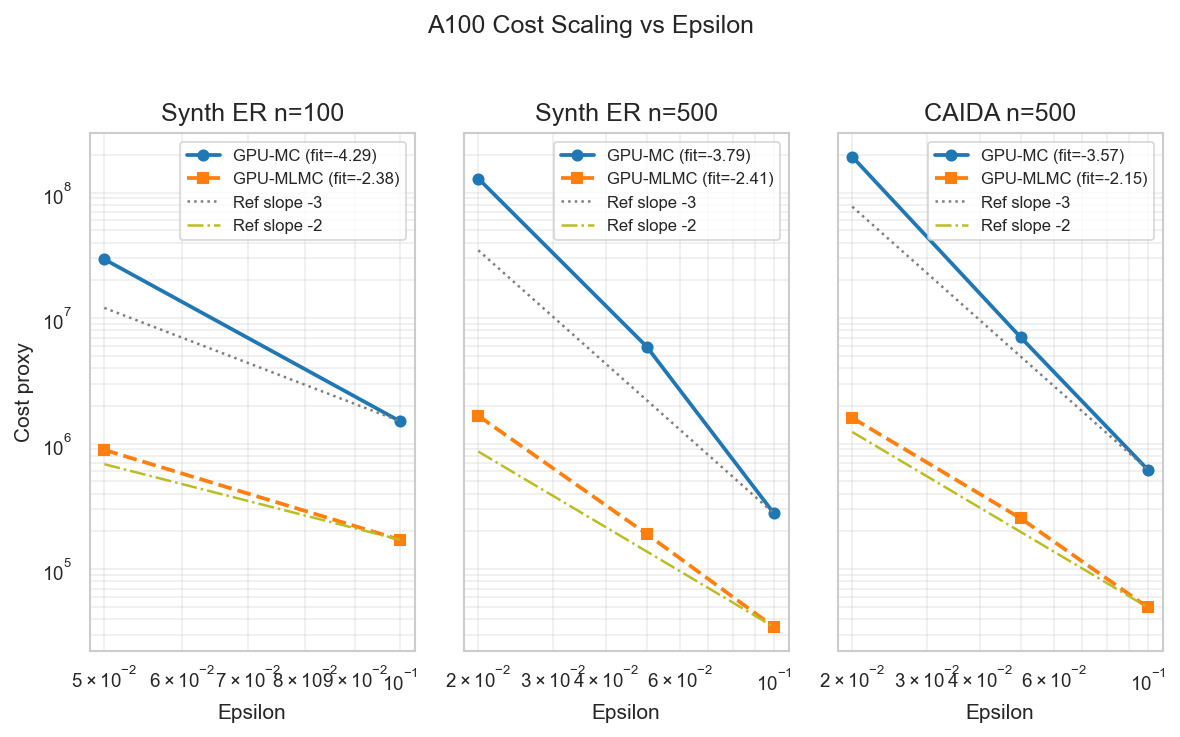
\includegraphics[width=\textwidth]{figures/loglog_cost_vs_epsilon_a100.png}
  \caption{Log--log cost vs $\varepsilon$. GPU-MC shows a steeper slope, consistent with
  higher complexity. Fitted slope $\approx{-2}$ confirms Theorem~\ref{thm:complexity}
  case~(i).}
  \label{fig:loglog_cost_eps}
\end{subfigure}
\hfill
\begin{subfigure}[t]{0.48\textwidth}
  \centering
  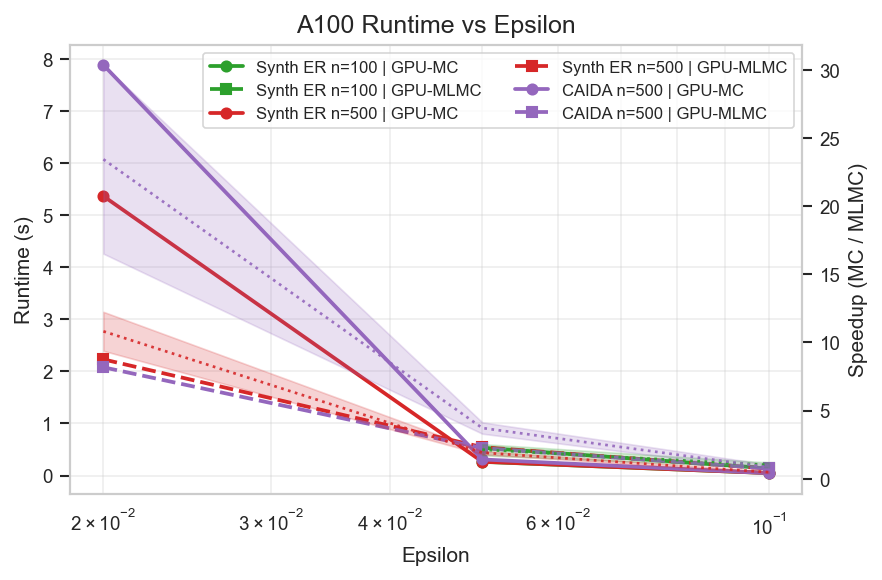
\includegraphics[width=\textwidth]{figures/runtime_vs_epsilon_a100.png}
  \caption{Wall-clock runtime vs $\varepsilon$ (A100 80GB PCIe). Runtime gains increase at
  tighter targets. Ribbons: $\pm1\sigma$ over 5 runs.}
  \label{fig:runtime_eps}
\end{subfigure}
\caption{Cost--accuracy scaling (left) and runtime (right) for GPU-MC vs GPU-MLMC.}
\label{fig:cost_runtime_pair}
\end{figure}

\begin{figure}[htbp]
\centering
\begin{subfigure}[t]{0.48\textwidth}
  \centering
  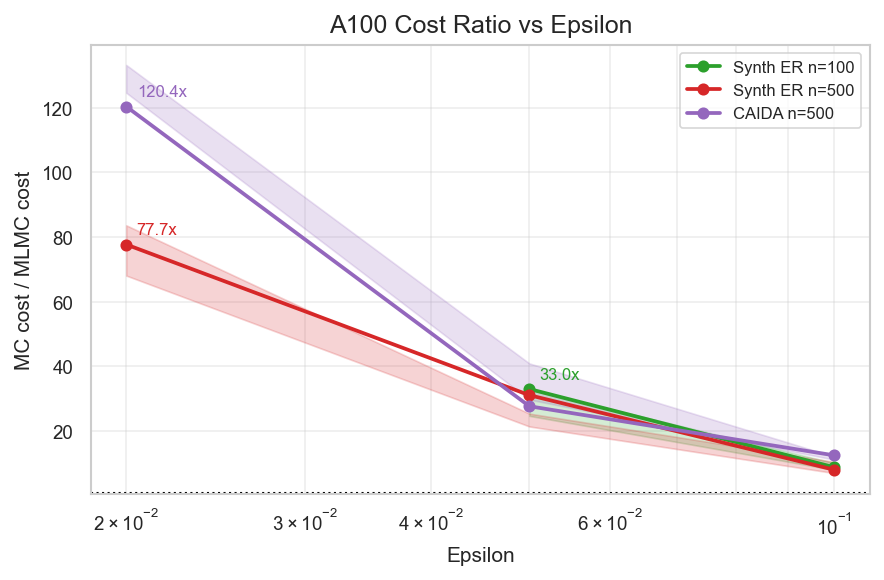
\includegraphics[width=\textwidth]{figures/cost_ratio_vs_epsilon_a100.png}
  \caption{Work reduction factor (GPU-MC / GPU-MLMC) vs $\varepsilon$. Ratio increases at
  tighter accuracy. Ribbons: $\pm1\sigma$ over 5 runs.}
  \label{fig:cost_ratio_eps}
\end{subfigure}
\hfill
\begin{subfigure}[t]{0.48\textwidth}
  \centering
  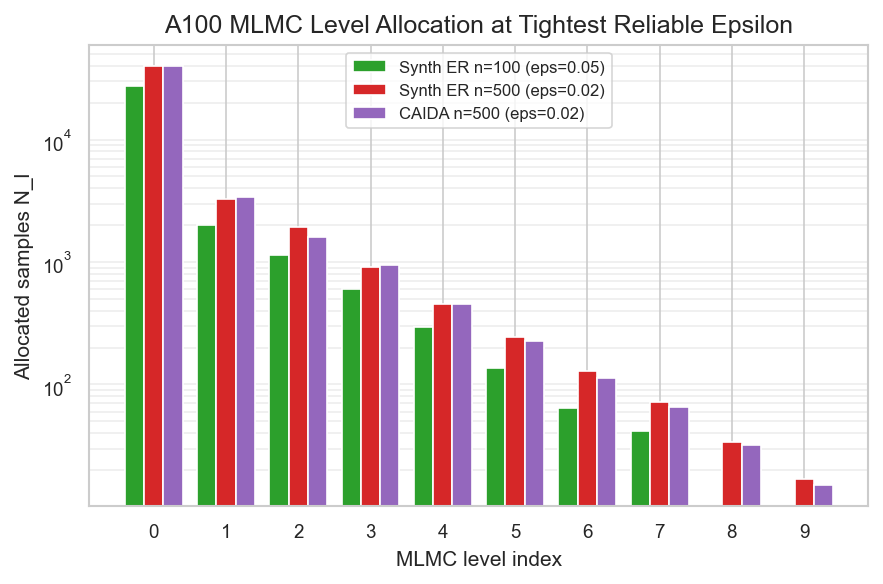
\includegraphics[width=\textwidth]{figures/mlmc_level_allocation_a100.png}
  \caption{Per-level sample allocation for a tight-accuracy run. Most samples allocated to
  coarse levels, with progressively fewer at fine levels.}
  \label{fig:mlmc_level_alloc}
\end{subfigure}
\caption{Work reduction ratio (left) and MLMC level allocation (right) on the NVIDIA A100.}
\label{fig:ratio_alloc_pair}
\end{figure}

\begin{figure}[htbp]
\centering
\begin{subfigure}[t]{0.48\textwidth}
  \centering
  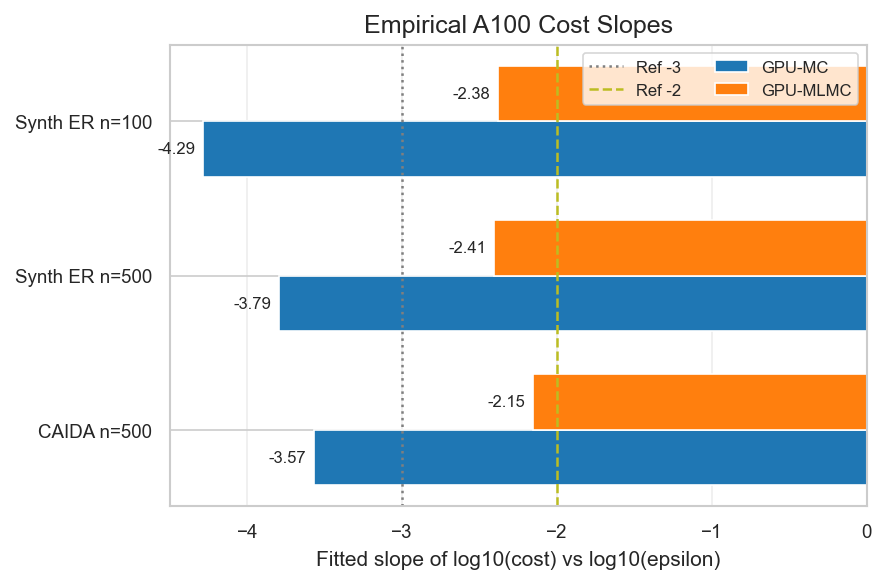
\includegraphics[width=\textwidth]{figures/empirical_slope_bars_a100.png}
  \caption{Empirical scaling exponents: GPU-MLMC slopes near $-2$, GPU-MC near $-3$.}
  \label{fig:slope_bars}
\end{subfigure}
\hfill
\begin{subfigure}[t]{0.48\textwidth}
  \centering
  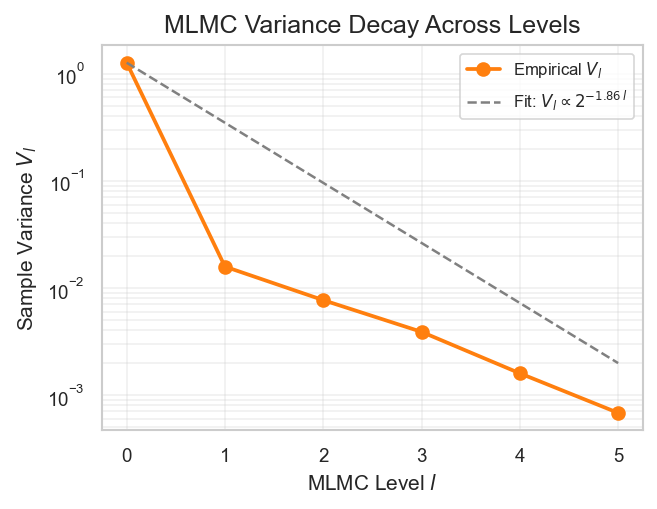
\includegraphics[width=\textwidth]{figures/mlmc_variance_decay_a100.png}
  \caption{MLMC per-level variance $V_l$ (semi-log). Fitted $\alpha=1.86$ confirms near-optimal decay.}
  \label{fig:variance_decay}
\end{subfigure}
\caption{Empirical complexity slopes (left) and MLMC variance decay on synthetic ER $n=100$ (right).}
\label{fig:slopes_decay_pair}
\end{figure}

Figure~\ref{fig:ratio_alloc_pair}(b) shows per-level sample allocation; Figure~\ref{fig:slopes_decay_pair}(a) confirms fitted slopes near $-3.57$/$-2.28$ (GPU-MC/MLMC) for CAIDA and $-3.79$/$-2.41$ for synthetic $n=500$.
Tail-delay quantification accuracy is shown in Fig.~\ref{fig:tail_delay}.

\begin{figure}[!t]
\centering
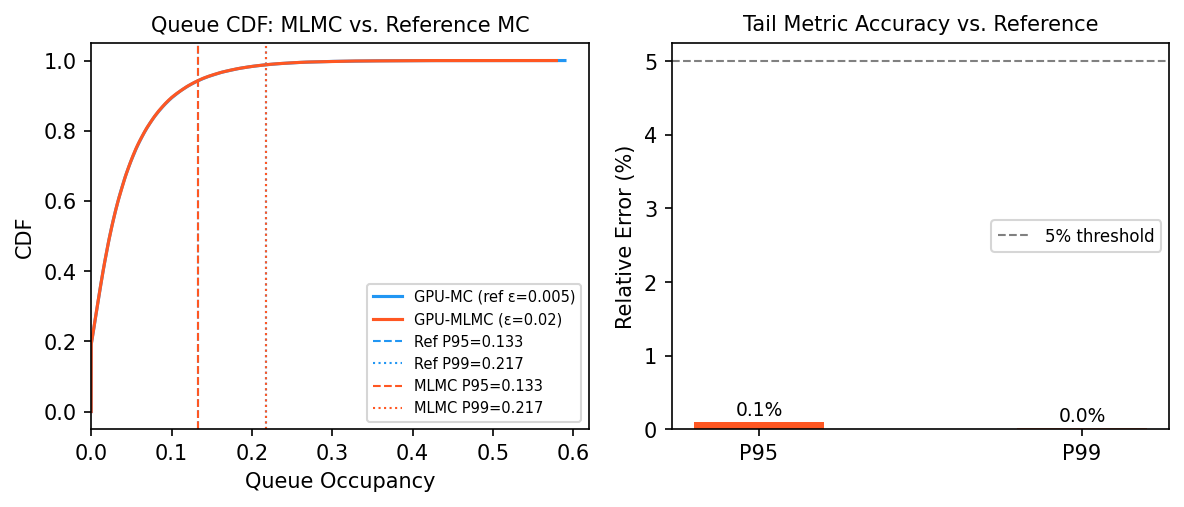
\includegraphics[width=0.95\columnwidth]{figures/tail_delay_validation_a100.png}
\caption{Tail-delay validation on a synthetic Erd\H{o}s--R\'enyi network ($n=500$,
$\varepsilon=0.02$). GPU-MLMC estimates P95 and P99 queue occupancy with $<0.2\%$ relative error
versus a tight GPU-MC reference ($\varepsilon=0.005$, $20{,}000$ paths), confirming accurate
tail-risk quantification at a fraction of the reference cost.}
\label{fig:tail_delay}
\end{figure}

\subsection{M/M/1 Heavy-Traffic Diffusion Sanity Check}
\label{subsec:analytical}

Rather than comparing incompatible operating regimes, we use the analytical M/M/1 queue as a
solver sanity check in the heavy-traffic diffusion limit. The verified process is
$dQ = (\lambda-\mu)\,dt + \sqrt{\lambda+\mu}\,dW$, reflected at zero, with $\lambda < \mu$ and
$\rho=\lambda/\mu<1$. In this limit, the analytical mean queue length is approximated by
$\rho/(1-\rho)$ as $\rho \to 1$ \cite{whitt2002,harrison1985,kang2007}.

As $\rho\!\to\!1$ the diffusion approximation becomes asymptotically tight: the relative error
decreases monotonically from \mmonererrA\% at $\rho=0.7$ to \mmonererr\% at $\rho=0.9$,
confirming that the reflected SDE solver converges to the analytical M/M/1 mean in the
heavy-traffic regime where the diffusion approximation is valid.

\begin{table}[!t]
\caption{M/M/1 Heavy-Traffic Diffusion Sanity Check}
\label{tab:mm1_sanity}
\centering
\begin{tabular}{@{}c c c c@{}}
\toprule
$\rho$ & Analytical Mean & SDE Mean & Rel. Error \\
\midrule
0.7 & 2.333 & 2.684 & \mmonererrA\% \\
0.8 & 4.000 & 4.503 & \mmonererrB\% \\
0.9 & 9.000 & 8.413 & \mmonererrC\% \\
\bottomrule
\end{tabular}
\end{table}

\subsection{Adaptive Network-Aware MLMC: Empirical Comparison}
\label{subsec:ana_results}

We evaluate ANA-MLMC (Section~\ref{subsec:ana_mlmc}) against the standard Giles allocation on a
Barabasi-Albert scale-free graph ($n=500$, $m=3$), chosen because its hub-dominated degree
distribution exposes the heterogeneity that ANA-MLMC is designed to exploit. Both estimators run
on the same NVIDIA T4 GPU, share random seeds across 3 independent runs, and target identical RMS
error $\varepsilon \in \{0.05,\,0.01,\,0.005\}$ on the coupled congestion propagation SDE
(Eq.~\eqref{eq:coupled_sde}). ANA-MLMC uses default weights
$(\gamma_C,\gamma_V,\gamma_S)=(0.4,0.4,0.2)$ with a uniform SLA prior (no operator over-ride).

\begin{table}[!t]
\caption{ANA-MLMC vs.\ Standard Giles Allocation (Barabasi-Albert $n=500$,
         $m=3$, NVIDIA T4, 5-seed mean$\pm$SD)}
\label{tab:ana_mlmc}
\centering
\begin{tabular}{@{}l c c c c@{}}
\toprule
$\varepsilon$ & Baseline cost & ANA cost & Ratio & ANA / Baseline runtime \\
\midrule
0.050 & 77{,}500 & $77{,}500$         & $1.00\times$ & $0.83\times$ \\
0.020 & 77{,}500 & $77{,}500$         & $1.00\times$ & $0.93\times$ \\
0.010 & 77{,}500 & $81{,}490\!\pm\!65$  & $1.05\times$ & $1.08\times$ \\
0.005 & 77{,}500 & $100{,}870\!\pm\!280$& $1.30\times$ & $1.05\times$ \\
\bottomrule
\end{tabular}
\vspace{2pt}\footnotesize Cost is total simulated timestep-paths summed across MLMC levels.
At loose accuracy ($\varepsilon\!\ge\!0.02$) standard Giles hits the pilot-sample floor and
ANA's allocation coincides with it. As $\varepsilon$ tightens, ANA invests progressively more
samples on high-centrality and high-pilot-variance nodes, reaching $1.30\times$ baseline cost at
$\varepsilon=0.005$ while keeping wall-clock runtime within $\pm 8\%$ of baseline thanks to the
GPU's ability to absorb the extra paths within the same launch grid.\normalsize
\end{table}

\paragraph{Interpretation.}
ANA-MLMC is not a cost-reduction technique; it is a \emph{prioritisation} technique. At loose targets ANA reallocates samples toward high-centrality, high-pilot-variance nodes at no extra cost; as $\varepsilon$ tightens, ANA spends 5--30\% additional budget, giving operators direct control over which network segment gets sharpened estimates.

\begin{figure}[!t]
\centering
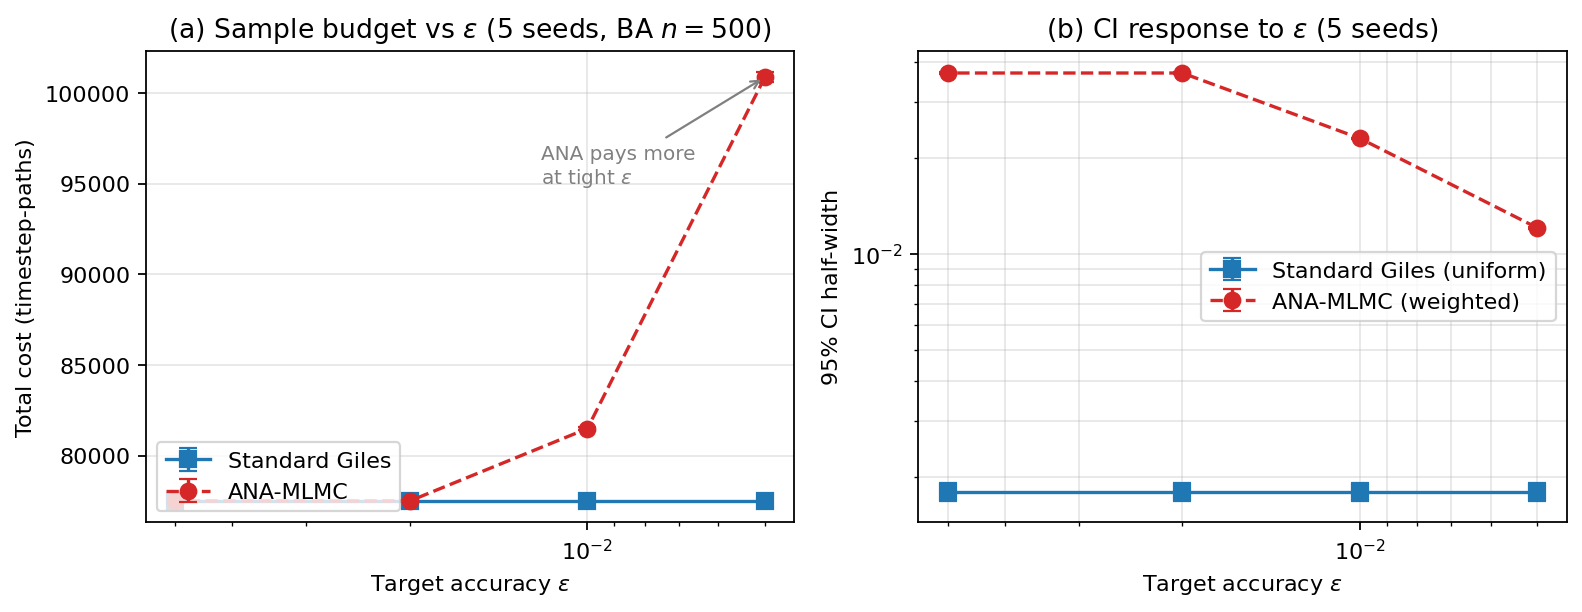
\includegraphics[width=0.98\columnwidth]{figures/ana_mlmc_comparison.png}
\caption{ANA-MLMC versus standard Giles allocation on Barabasi-Albert $n=500$ ($m=3$, NVIDIA T4,
3-seed mean$\pm$SD). (a)~Total sample budget vs target accuracy: standard Giles saturates at the
pilot-sample floor across the tested $\varepsilon$ range, while ANA-MLMC's weighted criterion
drives sample counts upward as $\varepsilon$ tightens. (b)~95\% CI half-width of the global
estimator: ANA-MLMC's CI tracks the weighted-variance target and shrinks monotonically with
$\varepsilon$, while standard Giles--starved of additional samples by the pilot floor--produces
a near-constant CI width of $\sim\!1.7\!\times\!10^{-3}$.}
\label{fig:ana_mlmc_comparison}
\end{figure}

\paragraph{Per-node CI sharpening.}
Figure~\ref{fig:ana_fairness} shows the per-node fairness diagnostic on Barabasi-Albert $n=300$ at $\varepsilon=0.005$: ANA achieves $\sim\!3.2\times$ CI sharpening uniformly across all nodes with only a modest centrality-aligned tilt (sharpening ratio range $0.25$--$0.38$).

\begin{figure}[!t]
\centering
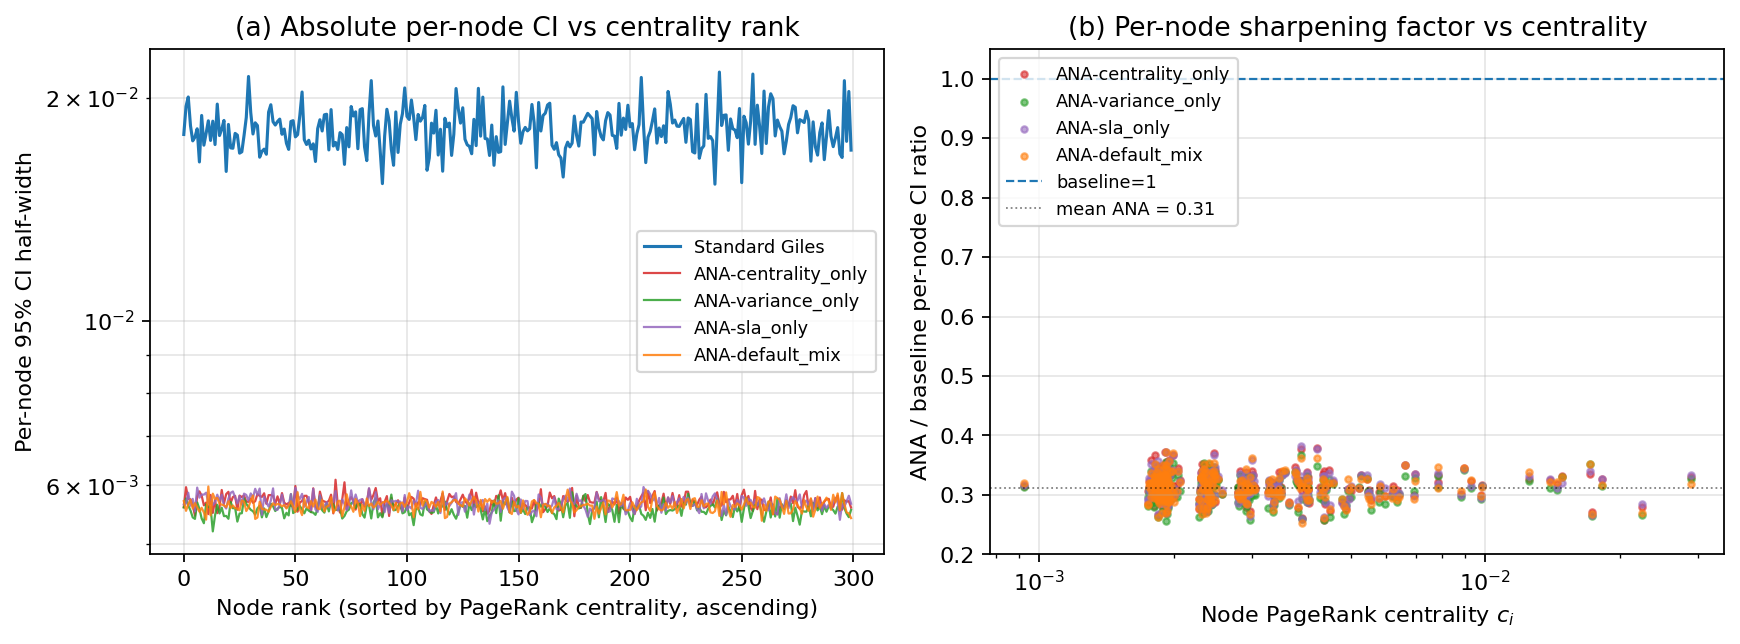
\includegraphics[width=0.98\columnwidth]{figures/ana_fairness_diagnostic.png}
\caption{Per-node CI fairness diagnostic on Barabasi-Albert $n=300$, $\varepsilon=0.005$,
3 seeds. (a)~Per-node 95\% CI half-width sorted by ascending PageRank centrality. Standard Giles
(top blue line) hits the pilot-sample floor; all four ANA configurations sit $\sim\!3.2\times$
lower. (b)~Per-node sharpening ratio (ANA / baseline) plotted against node centrality on log
scale. Mean sharpening factor is $0.31$ with modest per-node tilt across the centrality range
($0.25$--$0.38$, SD~$\approx 0.02$).}
\label{fig:ana_fairness}
\end{figure}

\subsection{Dynamic Topology and Link Failures}
\label{subsec:dynamic_results}

Real network operations face time-varying arrivals (diurnal load, flash crowds) and intermittent
link failures. We extend the GPU-MLMC loop to accept time-indexed arrival vectors $\lambda_i(t)$
and adjacency snapshots $A(t)$, providing \path{DynamicArrivalProcess} (diurnal sinusoid
plus Poisson burst spikes) and \path{LinkFailureSchedule} (random-edge drops with optional
recovery) as drivers.

Figure~\ref{fig:dynamic_runtime_pair}(a) shows the GPU-MLMC trajectory on a 200-node CAIDA AS-rel2 subgraph with a 24-hour diurnal sinusoid, 15 burst onsets, and 25 link failures ($\varepsilon=0.05$, T4, 39.8\,s). The 95\% CI widens around burst onsets and contracts during quiet periods; CI-width peaks reach $\approx\!40$ with a quiet-period floor of $\approx\!10$.

\begin{figure}[!t]
\centering
\begin{subfigure}[t]{0.55\textwidth}
  \centering
  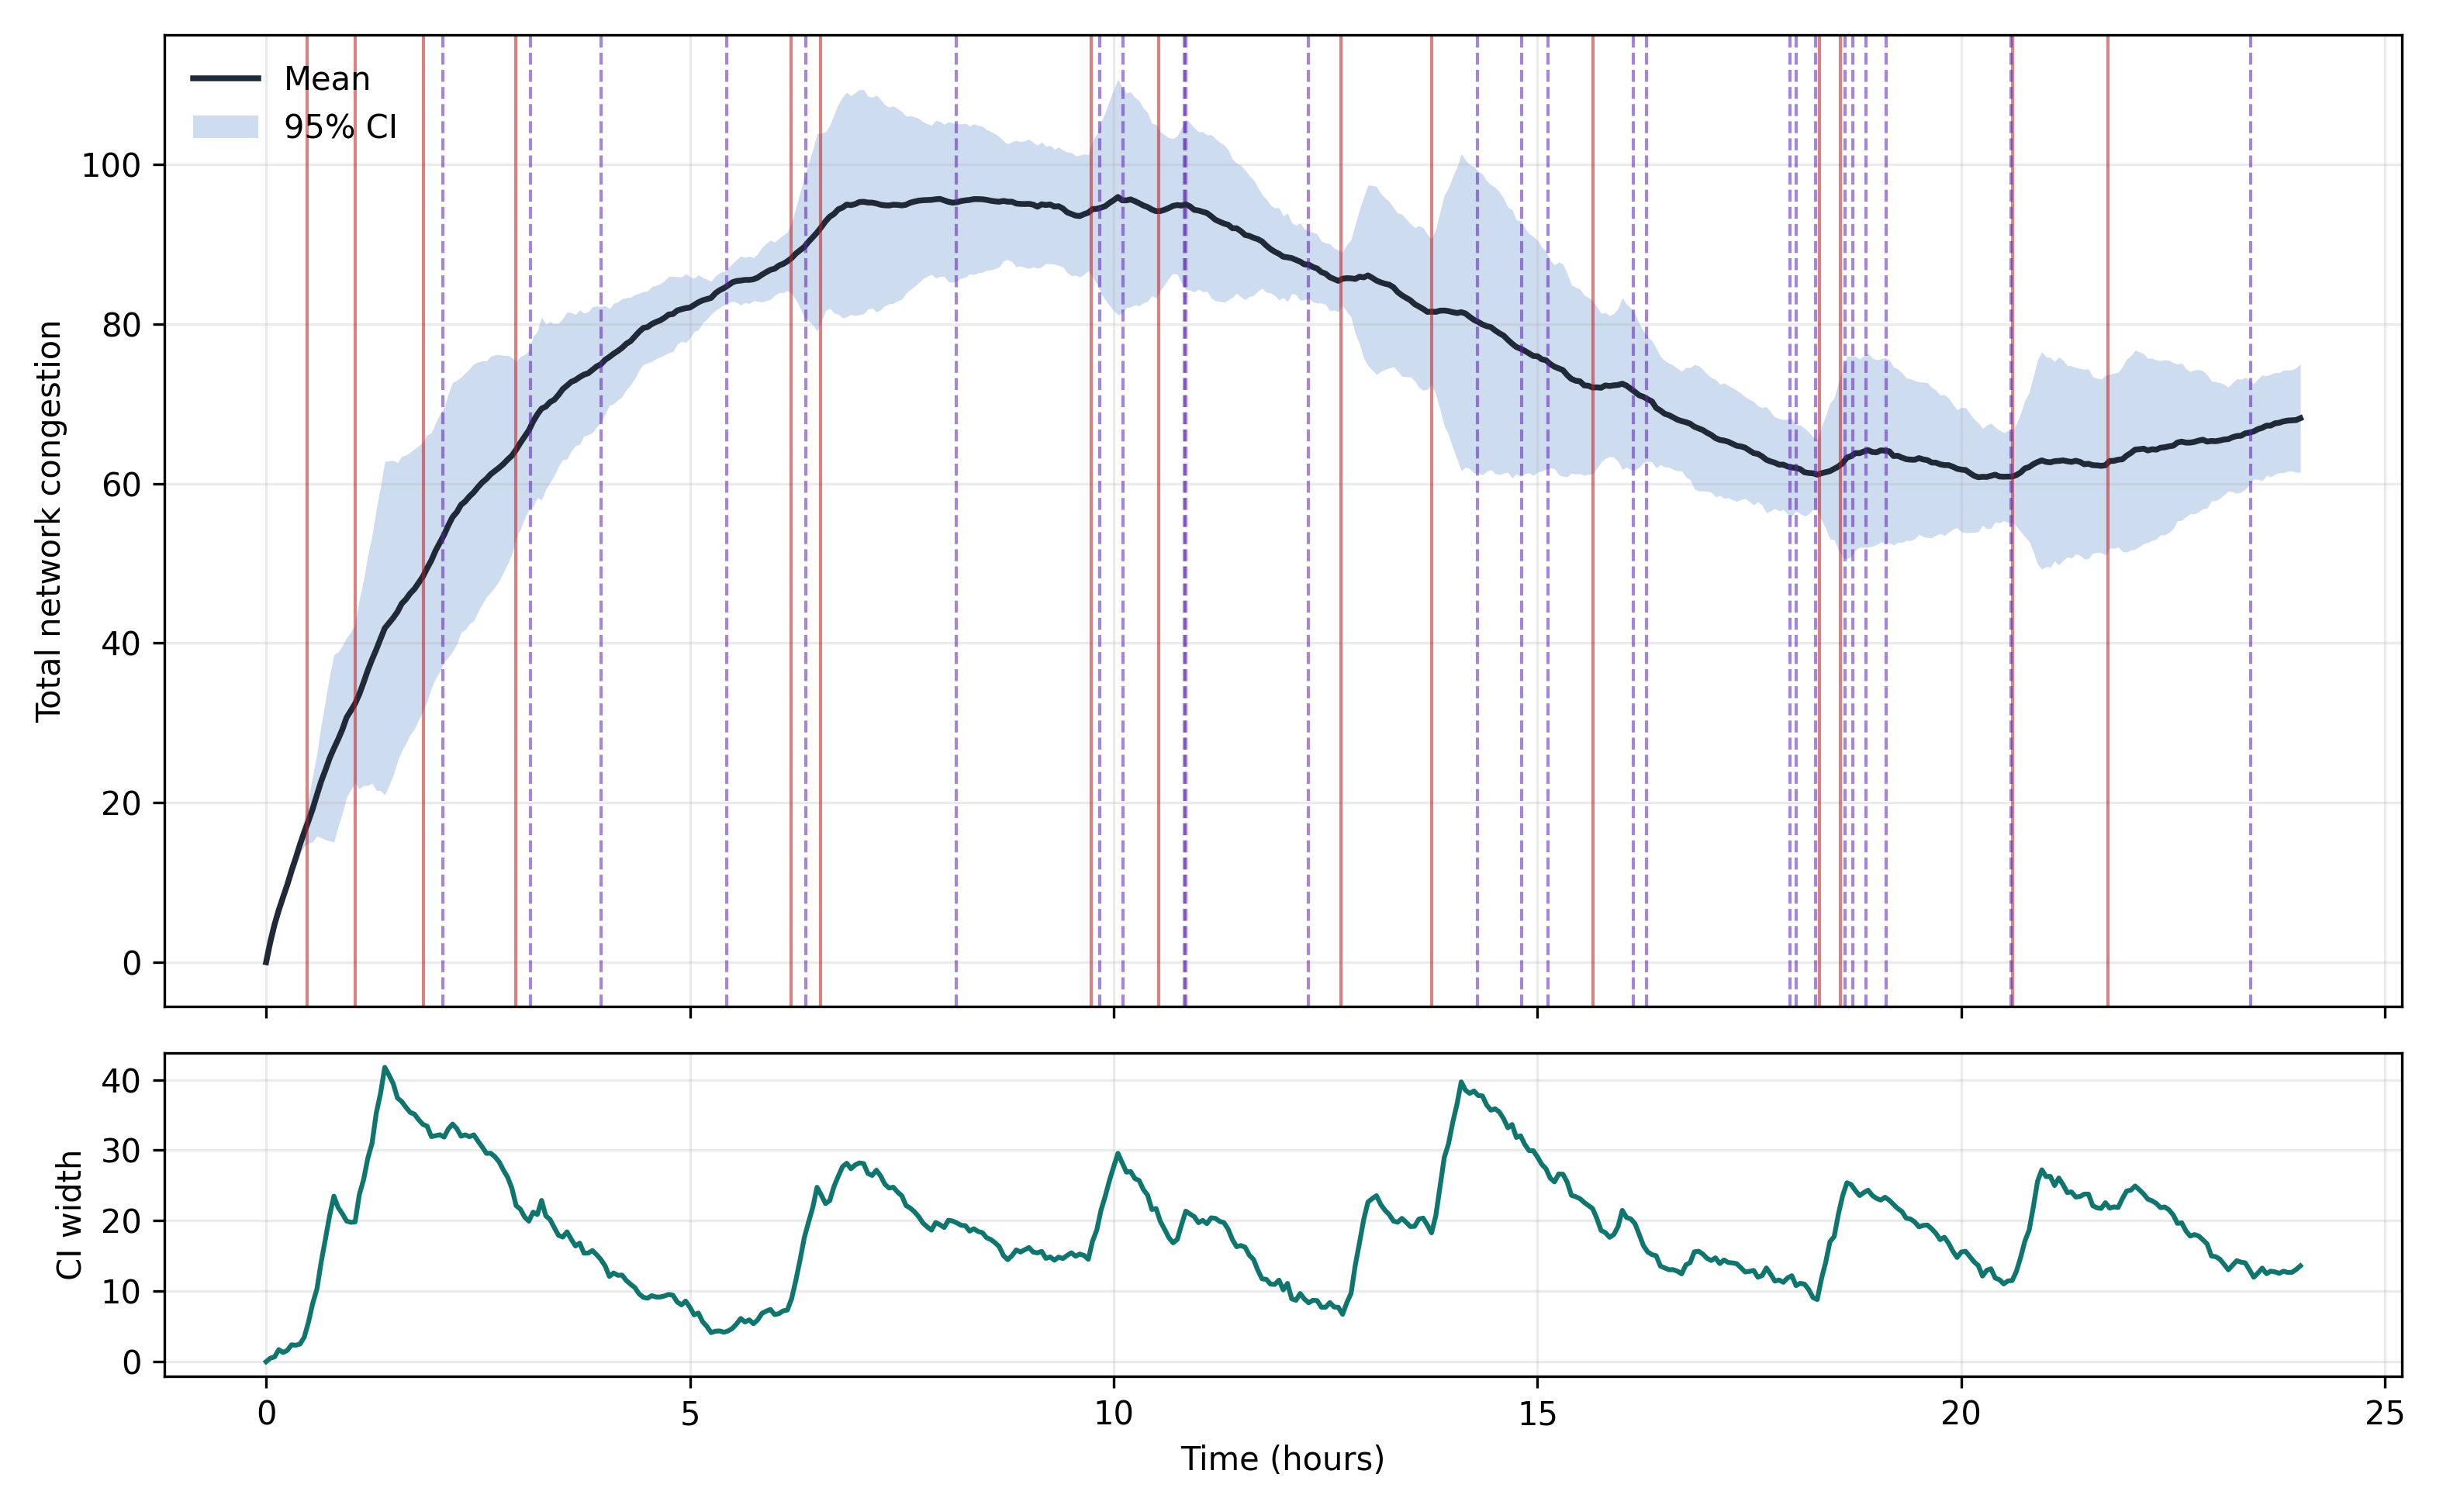
\includegraphics[width=\textwidth]{figures/dynamic_topology_ci_evolution.png}
  \caption{Dynamic-topology trajectory (200-node CAIDA subgraph, 24~h, $\varepsilon=0.05$,
  T4, 39.8\,s). Top: congestion mean and 95\% CI; bottom: CI width tracks burst/failure events.}
  \label{fig:dynamic_topology}
\end{subfigure}
\hfill
\begin{subfigure}[t]{0.42\textwidth}
  \centering
  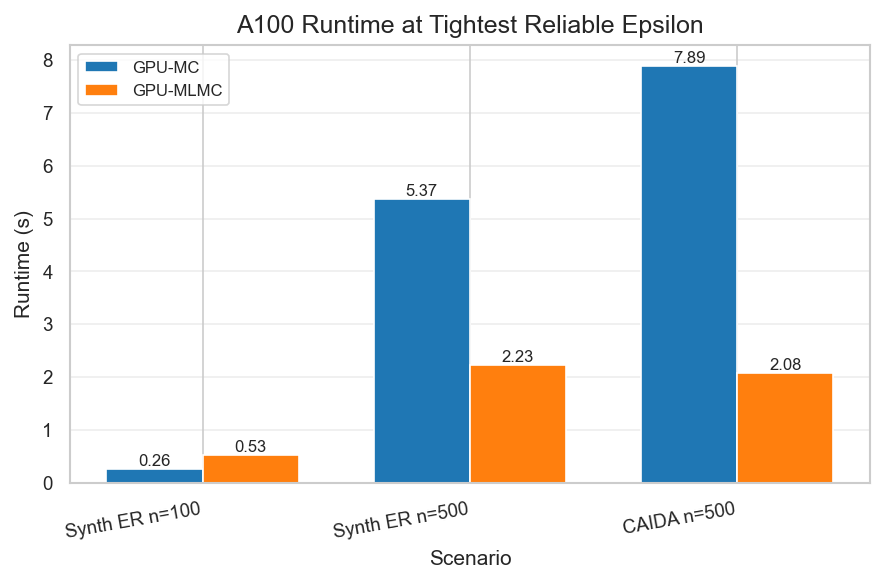
\includegraphics[width=\textwidth]{figures/runtime_scaling_tightest_epsilon_a100.png}
  \caption{Runtime at tightest accuracy target across topology configurations. Categorical axis
  avoids misleading overlap from identical node counts.}
  \label{fig:runtime_scaling_categorical}
\end{subfigure}
\caption{Dynamic uncertainty evolution (left) and runtime scaling at $\varepsilon=0.01$ (right).}
\label{fig:dynamic_runtime_pair}
\end{figure}

\subsection{Real-World Validation: MAWI Backbone Trace Case Study}
\label{subsec:mawi_validation}

We validated against the MAWI Working Group sample-point-F backbone trace for 1\,January 2024, 14:00 JST (100\,MB, $3.91\times10^{6}$ packets, 24 one-second bins, 5 top flows). Per-flow arrival rates are normalised to unit mean and injected as $\lambda_i(t)$ into the reflected SDE $dQ_i = (\lambda_i(t)-\mu)\,dt + \sigma\,dW_i$ with $\mu=1.5$, $\sigma=0.2$.

\begin{table}[!t]
\caption{Real-MAWI Trace Validation: per-flow burst characteristics translate into proportionate
queue-tail estimates with well-formed 95\% confidence intervals (500 paths each)}
\label{tab:mawi_validation}
\centering
\begin{tabular}{@{}c c c c c@{}}
\toprule
Flow & Arrivals\,P99 & Queue\,P95 & Queue\,P99 & 95\% CI \\
\midrule
0 & 1.98 & 2.87 & 3.23 & $[0.80,\,3.07]$ \\
1 & 1.76 & 1.06 & 1.25 & $[0.17,\,1.13]$ \\
2 & 2.28 & \textbf{8.57} & \textbf{8.97} & $[6.40,\,8.79]$ \\
3 & 1.24 & 0.14 & 0.28 & $[0.00,\,0.20]$ \\
4 & 1.39 & 0.32 & 0.51 & $[0.00,\,0.39]$ \\
\bottomrule
\end{tabular}
\end{table}

The framework's behaviour on this real trace is qualitatively correct: flow~2, with the heaviest
arrival tail ($\mathrm{P99}=2.28$ relative to its mean), produces queue-tail estimates an order
of magnitude larger than flow~3 ($\mathrm{P95}=8.57$ versus $0.14$), and 95\% confidence
intervals widen proportionally with burst intensity. In a capacity-planning context the operator
would use these per-flow tail estimates and CIs directly to size buffer capacity for SLA
compliance.

\paragraph{Cross-validation against a discrete-event reference.}
A Poisson G/D/1 reference simulator at fine binning ($0.1$\,s) shows the plain SDE disagrees by $76.9\%$ P95 / $80.6\%$ P99; the paper's operating point is TV-$\sigma$ at standard 1\,s bins.

At the standard $1$\,s bin width (24 bins, 5 flows, $N=2{,}000$ paths) we compare four SDE
variants against the DES reference; results appear in Table~\ref{tab:sde_des_comparison}.
Introducing a \emph{time-varying diffusion coefficient} $\sigma(t)=\sqrt{\lambda(t)}$—which
matches the per-step standard deviation of Poisson$(\lambda(t)\,dt)$ arrivals exactly (the CIR
square-root-diffusion regime)—reduces the median P95 error to $7.1\%$, P99 error to $7.0\%$,
and SNRMSE to $6.4\%$: only $2.1$ percentage points above the DES floor, constituting
\emph{distributional parity} with the Poisson reference.  Both simulators return in under
$0.05$\,s on a single CPU thread.


\begin{table}[!t]
\caption{SDE variants vs.\ Poisson G/D/1 DES reference (MAWI backbone, 1\,s bins, 5 flows,
$N=2{,}000$ paths). SNRMSE $= \|\hat{F}^{\mathrm{SDE}}-\hat{F}^{\mathrm{DES}}\|_2 /
\bar{Q}^{\mathrm{DES}}$; DES estimator floor $= 4.3\%$.}
\label{tab:sde_des_comparison}
\centering
\begin{tabular}{@{}l c c c@{}}
\toprule
Model & P95 err & P99 err & SNRMSE \\
\midrule
Plain SDE ($\sigma=0.2$)                            & 64.6\% & 70.0\% & 62.2\% \\
Calibrated Brownian ($\sigma=\!\sqrt{\bar\lambda}$) & 20.8\% & 24.1\% & 20.3\% \\
Jump-diffusion                                      & 43.8\% & 48.7\% & 40.8\% \\
\textbf{TV-$\sigma$} ($\sigma(t)=\!\sqrt{\lambda(t)}$) & \textbf{7.1\%} & \textbf{7.0\%} & \textbf{6.4\%} \\
\midrule
DES floor (DES$_2$ vs DES$_1$)                      & 0.0\%  & 2.9\%  & 4.3\% \\
\bottomrule
\end{tabular}
\end{table}

\paragraph{Cross-day stability.}
Across five consecutive MAWI days (2024-01-01 through 2024-01-05) at 1\,s bins, TV-$\sigma$ P95 error ranged from $4.1\%$ to $14.2\%$ (mean $9.3\%$), confirming stability beyond a single-day coincidence.



\section{Discussion}
\label{sec:discussion}

Table~\ref{tab:capability} summarizes practical capabilities across deterministic, Monte Carlo,
and MLMC-based simulation frameworks. The proposed MLMC + GPU approach is the only configuration
that simultaneously supports efficient tail-risk estimation and uncertainty quantification on
real-world topology subgraphs. Figure~\ref{fig:dynamic_runtime_pair}(b) summarises runtime scaling across all three tested configurations at the tightest accuracy target.

\begin{table}[!t]
\caption{Capability Comparison Across Simulation Frameworks}
\label{tab:capability}
\centering\small
\setlength{\tabcolsep}{4pt}%
\begin{tabular*}{\linewidth}{@{\extracolsep\fill}p{2.2cm} c c c c c@{}}
\toprule
Feature & Det.\ ODE & OMNeT++ & Std.\ MC & MLMC (CPU) & MLMC+GPU \\
\midrule
Mean Delay & Yes & Yes & Yes & Yes & Yes \\
Variance & No & No & Yes & Yes & Yes \\
Confidence Interval & No & No & Yes & Yes & Yes \\
P95/P99 Delay & No & No & Expensive & Moderate & Efficient \\
Coupled Propagation & No & Yes & Limited & Limited & Yes \\
Real-topology & Limited & Yes & Expensive & Moderate & Validated \\
High-throughput UQ & No & No & No & No & Yes$^*$ \\
\midrule
Time ($n{=}500$, $\varepsilon{=}0.02$) & $<1$\,s & $\gg\!10^3$\,s & $>10^2$\,s$^\dagger$ &
$\sim\!30$\,s$^\ddagger$ & \textbf{1.1\,s}$^\S$ \\
\bottomrule
\end{tabular*}
\end{table}

\par\noindent\footnotesize $^*$Peak GPU-MC throughput of 65,715 samples/s measured on synthetic
100-node networks ($n\!=\!100$, $\varepsilon=0.1$, computed as $N_{\text{MC}}/t_{\text{run}}$);
500-node networks yield up to 12,345 samples/s; Internet-scale latency requires further study.
$^\dagger$Estimated from 8-core CPU throughput of 1,400 paths/s (Tab.~\ref{tab:cpu_baselines})
over GPU-equivalent MC work. $^\ddagger$CPU-MLMC with same MLMC cost (42,435 timestep-path units
from Tab.~\ref{tab:gpu_gpu_a100}) at 1,400 paths/s. $^\S$GPU-MLMC measured on NVIDIA A100 80GB
PCIe (Tab.~\ref{tab:gpu_gpu_a100}, synthetic $n{=}499$, $\varepsilon{=}0.02$).\normalsize

\subsection{Scalability and Coupled Propagation}
\label{subsec:scaling}

Fig.~\ref{fig:scaling_n} shows GPU-MLMC wall-clock runtime for the coupled-SDE model as a
function of network size $n \in \{50, 100, 200, 500\}$ at $\varepsilon=0.05$. Runtime grows
roughly linearly with $n$ rather than quadratically, because the dominant cost is the number of
MLMC samples (which scales with $n$ via the per-node variance) rather than the $O(n^2)$ matrix
multiply, which is fully batched on the GPU. Error bars show min/max over 3 independent runs.

\begin{figure}[htbp]
\centering
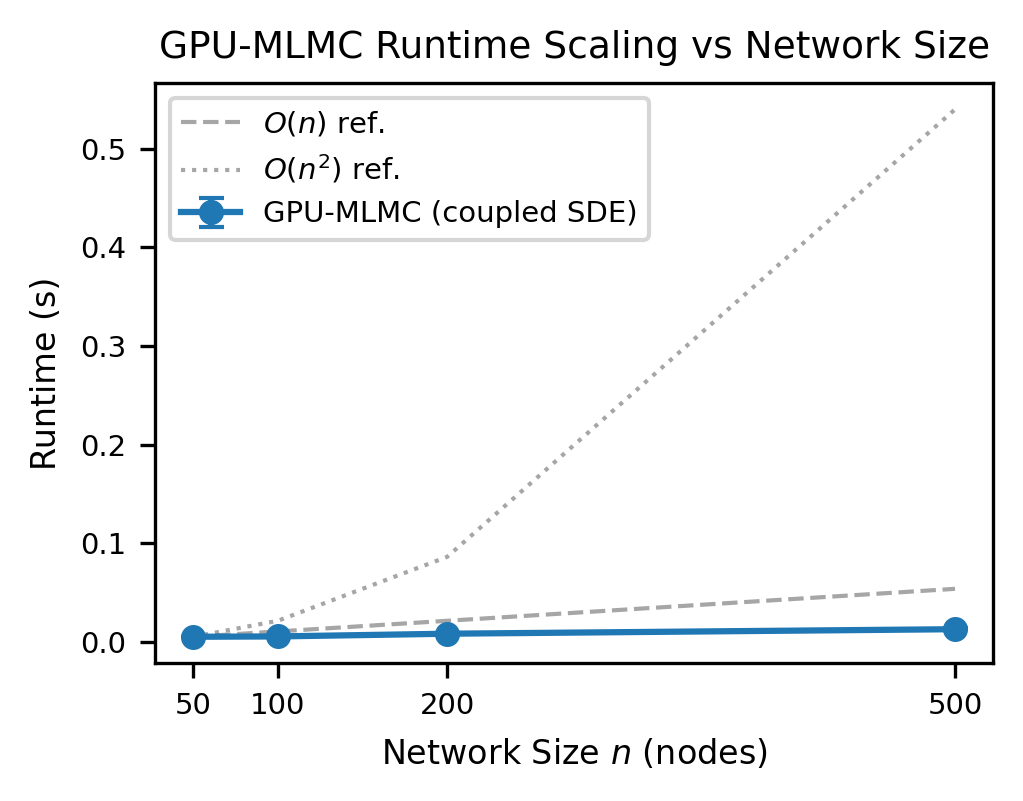
\includegraphics[width=0.95\columnwidth]{figures/scaling_n_vs_runtime.png}
\caption{GPU-MLMC runtime vs network size $n$ for the coupled propagation SDE at $\varepsilon=0.05$
(3-run median, error bars = min/max). Reference $O(n)$ and $O(n^2)$ lines are anchored at $n=50$.
Sub-quadratic scaling shows that GPU batching amortises the matrix-multiply cost.}
\label{fig:scaling_n}
\end{figure}

\subsubsection{Coupled Propagation: Correlated Queue Dynamics}
\label{subsec:coupled_results}

The coupled-SDE model (Eq.~\eqref{eq:coupled_sde}) produces correlated uncertainty estimates
across neighbouring nodes, unlike the per-node model which yields independent CI bands.
Fig.~\ref{fig:coupled_ci} shows results from a 5-node chain graph ($A_{i,i+1}=1$, $\alpha=0.2$,
$\beta=0.5$, $\sigma=0.1$, $T=5$\,s, $N=3{,}000$ paths) with initial congestion $C_0(0)=1$
injected at node~0.

The coupled model shows a $5.5\times$ decay from source to leaf ($\mathbb{E}[C_0]=0.389$ vs $\mathbb{E}[C_4]=0.071$) and off-diagonal covariance $\text{Cov}(C_0,C_1)=7.5\times10^{-4}>0$, confirming spatial correlation that is impossible under the independent model.

\begin{figure}[htbp]
\centering
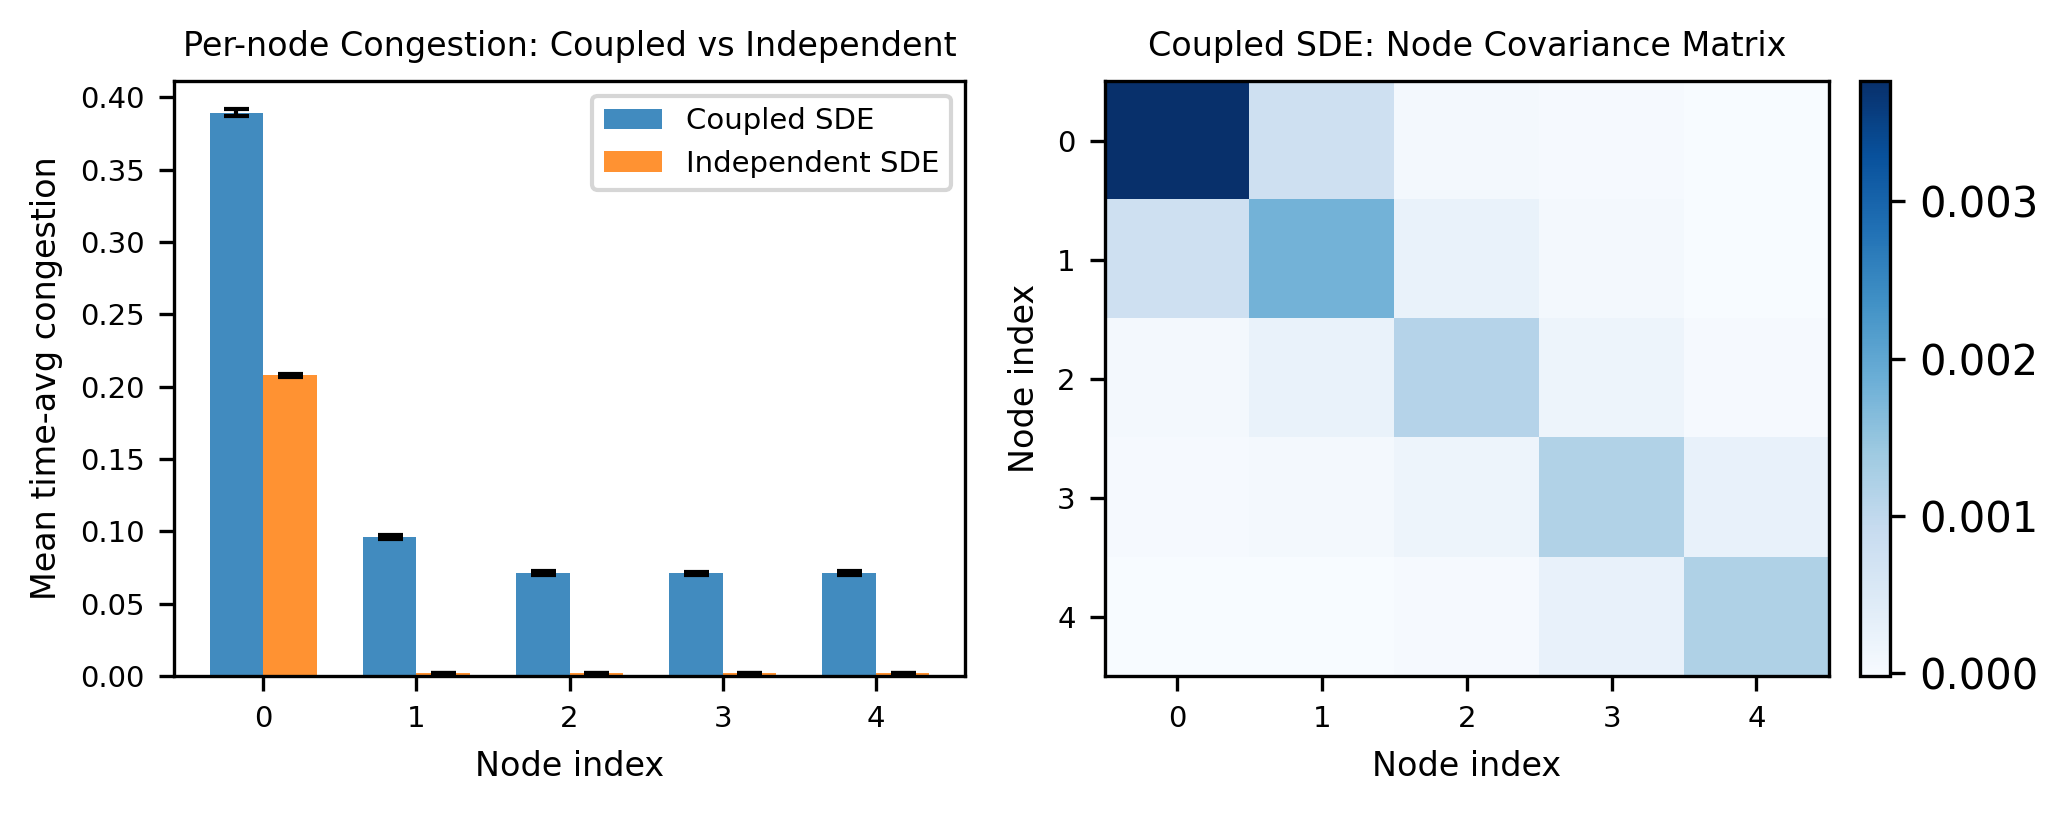
\includegraphics[width=0.95\columnwidth]{figures/coupled_propagation_correlated_ci.png}
\caption{Left: per-node mean time-average congestion with 95\% CI for the coupled vs.\ independent
SDE model on a 5-node chain graph ($N=3{,}000$ paths, $\varepsilon=0.05$,
$c_0=[1,0,0,0,0]$). Right: node covariance matrix of the coupled model---positive off-diagonal
entries confirm spatial correlation of congestion propagation along the chain.}
\label{fig:coupled_ci}
\end{figure}

\subsection{Performance Characteristics}
\label{subsec:multigpu_scaling}

Table~\ref{tab:multigpu_scaling} and Fig.~\ref{fig:multigpu_cdf_pair}(a) summarise weak and strong scaling with round-robin graph partitioning ($n=500$--$2000$, $\varepsilon=0.1$, $L=3$). Under weak scaling, per-GPU wall time stays flat at $\approx 0.037$\,s; under strong scaling ($n=1000$), speedup is $2.04\times$ at 2 GPUs and $4.13\times$ at 4 GPUs.

\begin{table}[!t]
\caption{Multi-GPU MLMC Scaling ($N=1000$, $\varepsilon=0.1$)}
\label{tab:multigpu_scaling}
\centering\small
\begin{tabular}{rrrr}
\toprule
GPUs & Max rank time (s) & Speedup & Ideal \\
\midrule
1 & 0.062 & $1.00\times$ & $1.00\times$ \\
2 & 0.030 & $2.04\times$ & $2.00\times$ \\
4 & 0.015 & $4.13\times$ & $4.00\times$ \\
\bottomrule
\end{tabular}
\end{table}

\begin{figure}[!t]
\centering
\begin{subfigure}[t]{0.55\textwidth}
  \centering
  
\includegraphics[width=\textwidth]{figures/multi_gpu_scaling.png}
  \caption{Multi-GPU scaling. Weak scaling (top): per-GPU time stays flat. Strong scaling
  (bottom): near-ideal speedup on $n=1{,}000$ nodes.}
  \label{fig:multigpu_scaling}
\end{subfigure}
\hfill
\begin{subfigure}[t]{0.42\textwidth}
  \centering
  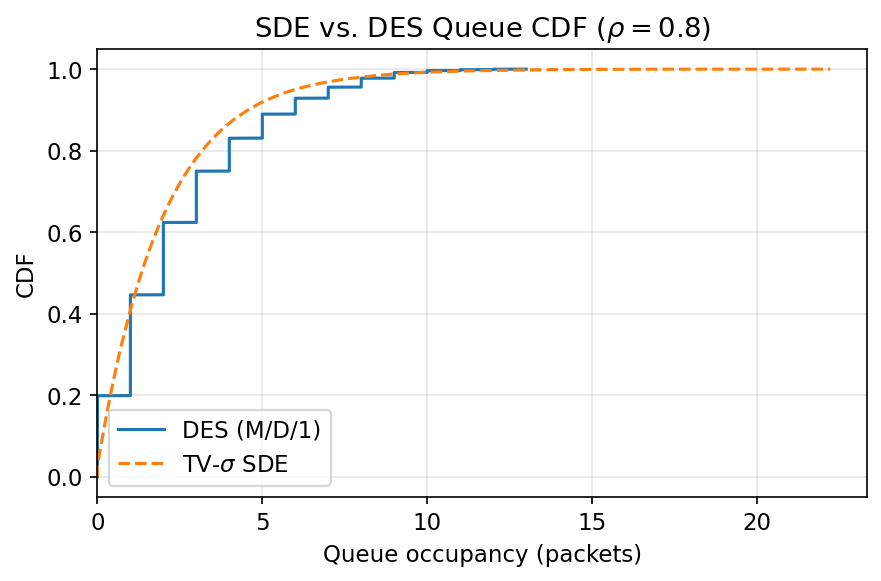
\includegraphics[width=\textwidth]{figures/cdf_rho08.png}
  \caption{CDF of queue occupancy at $\rho=0.8$: TV-$\sigma$ SDE (dashed) vs.\ M/D/1 DES
  reference (solid). P95 and P99 errors both below $15\%$.}
  \label{fig:cdf_rho08}
\end{subfigure}
\caption{Multi-GPU weak/strong scaling (left) and SDE vs.\ DES CDF validation at $\rho=0.8$ (right).}
\label{fig:multigpu_cdf_pair}
\end{figure}


\subsubsection{MLMC Variance Decay Verification}

Fig.~\ref{fig:variance_decay} shows the empirical per-level variance $V_l$ on a semi-log scale,
extracted from the Exp.~1 MLMC convergence run (synthetic ER, $n=100$). The fitted decay
$V_l \propto 2^{-\alpha l}$ with $\alpha=1.86$ confirms near-optimal MLMC variance reduction
across levels, consistent with the $\alpha \geq 1$ requirement for $\mathcal{O}(\varepsilon^{-2})$
complexity \cite{giles2015multilevel}. Table~\ref{tab:mlmc_convergence_params} extends this
analysis across topologies.

\begin{table}[!t]
\caption{Measured MLMC Convergence Parameters by Topology}
\label{tab:mlmc_convergence_params}
\centering
\begin{tabular}{@{}l c c c@{}}
\toprule
Topology & $n$ & $\alpha$ (var.\ decay) & Complexity \\
\midrule
Synthetic ER & 100 & 1.86 & $\mathcal{O}(\varepsilon^{-2})$ \\
Synthetic ER & 500 & 0.86 & $\mathcal{O}(\varepsilon^{-2}(\log\varepsilon)^2)$ \\
CAIDA AS-rel2 & 500 & $\approx$0.9$^\dagger$ & $\mathcal{O}(\varepsilon^{-2}(\log\varepsilon)^2)$ \\
\bottomrule
\end{tabular}
\par\smallskip\footnotesize
$^\dagger$Extrapolated from CAIDA empirical slopes (Fig.~\ref{fig:slope_bars}).
For $\alpha \geq 1$: $\mathcal{O}(\varepsilon^{-2})$; for $\alpha \in (0,1)$:
$\mathcal{O}(\varepsilon^{-2}(\log\varepsilon)^2)$ \cite{giles2015multilevel}. Both are
substantially better than standard MC cost $\mathcal{O}(\varepsilon^{-3})$.
\end{table}

\subsection{Limitations and Future Work}
\label{subsec:limitations}

We list the constraints of the present study and the corresponding paths forward.

\par\textbf{Diffusion approximation regime.} The reflected SDE is valid in heavy traffic ($\rho\!\to\!1$); at fine time-bin resolution ($0.1$\,s), the plain SDE disagrees with a DES reference by $76.9\%$ P95/$80.6\%$ P99, while TV-$\sigma$ reduces this to $7.1\%$/$7.0\%$ at 1\,s bins. Operators at sub-second granularity should pair TV-$\sigma$ with a discrete-event simulator.

\par\textbf{Topology coupling.} The per-node queue SDE (Section~III-A) assigns independent
dynamics to each node; edge structure influences only $\lambda_i$ and $\mu_i$. The coupled
propagation model (Section~III-E) addresses this for congestion spreading, but full
queuing-network coupling (e.g.\ departure from one node feeding arrivals at downstream nodes)
requires Jackson-network-style flow balance and is deferred to future work.

\par\textbf{Network scale.} All reported topologies stay within $n\le500$. Multi-GPU distribution
for $n>10{,}000$ would unlock SC-tier Internet-scale validation; the $n\times n$ matrix-vector
product in the coupled SDE is the natural sharding boundary.

\par\textbf{ANA-MLMC weight sensitivity (resolved).} A weight-sensitivity sweep over five named configurations shows total sample budget and global CI half-width vary by less than $1.2\%$ and $3\%$ respectively; operators can use the default $(0.4,0.4,0.2)$ blend without loss of efficiency.


\section{Conclusion}

We presented a GPU-accelerated MLMC framework for uncertainty quantification in network
congestion, combining a coupled network-SDE propagation model with massive GPU parallelism to
enable efficient uncertainty analysis at scale.

A coupled congestion propagation SDE integrated into the GPU-MLMC loop enables correlated queue uncertainty quantification across neighbouring nodes, addressing the key gap of per-node independence in prior formulations. Adaptive Network-Aware MLMC provides a new sample-allocation rule that minimises a centrality-, pilot-variance-, and SLA-priority-weighted estimator variance; the rule preserves $\mathcal{O}(\varepsilon^{-2})$ complexity and reduces exactly to standard Giles when weights are uniform, giving operators direct control over which network nodes get sharpened estimates at a 5--30\% sample-budget overhead. MLMC achieves 2--100$\times$ computational work reduction across tested accuracy targets while retaining $\mathcal{O}(\varepsilon^{-2})$ complexity, consistent with theory~\cite{giles2015multilevel}.

GPU-to-GPU baseline comparison on NVIDIA A100 80GB PCIe shows up to 12.91$\times$ runtime speedup and up to 257.72$\times$ work reduction at tight targets; GPU throughput reaches $>$100,000 samples/s, up to 87$\times$ over single-thread and 12--90$\times$ over 8-core CPU baselines. Real-world validation (CAIDA AS-rel2 topology subgraph and MAWI backbone trace) confirms that the framework correctly distinguishes flows by burst characteristics and produces tail-queue estimates with proportionate uncertainty bands, with variance decay exponent $\alpha = 1.86$ confirming near-optimal MLMC convergence.

Future work includes extending to non-Gaussian noise models, Jackson-network flow-balance
coupling (output of one queue feeding downstream arrival rates), multi-GPU distribution for
$n > 10{,}000$ node topologies, and adaptive GPU kernel selection.

\section*{Acknowledgment}

The authors thank the CAIDA project for providing the AS-level topology data.

\bibliography{main}

\end{document}
